\documentclass[11pt, a4paper]{report}
\usepackage{graphicx}
\usepackage[table,xcdraw]{xcolor}
\usepackage{geometry}
\usepackage[backend=biber]{biblatex}
\usepackage{float}
\usepackage{authblk}
\usepackage{anyfontsize}
\usepackage[document]{ragged2e}
\usepackage{titlesec}
\usepackage[parfill]{parskip}
\titleformat{\chapter}[hang] 
{\normalfont\huge\bfseries}{\chaptertitlename\ \thechapter:}{1em}{} 
\geometry{left=2.5cm,right=2.5cm,top=2.5cm,bottom=2.5cm}
\graphicspath{ {./images/} }

\addbibresource{bibfolder/ref.bib}

% CHECK https://www.youtube.com/watch?v=ZYvS52511oQ FOR INFO ON SETTINGS FOR biblatex

\begin{document}

\pagestyle{empty}
\centering
\fontsize{2cm}{2cm}\selectfont{Research document} \\
\vspace{2mm}
\fontsize{1cm}{1cm}\selectfont Audio digital signal processor \\
\vspace{2mm}
\large BeCreative Minor\\
\normalsize
\vspace{4cm}
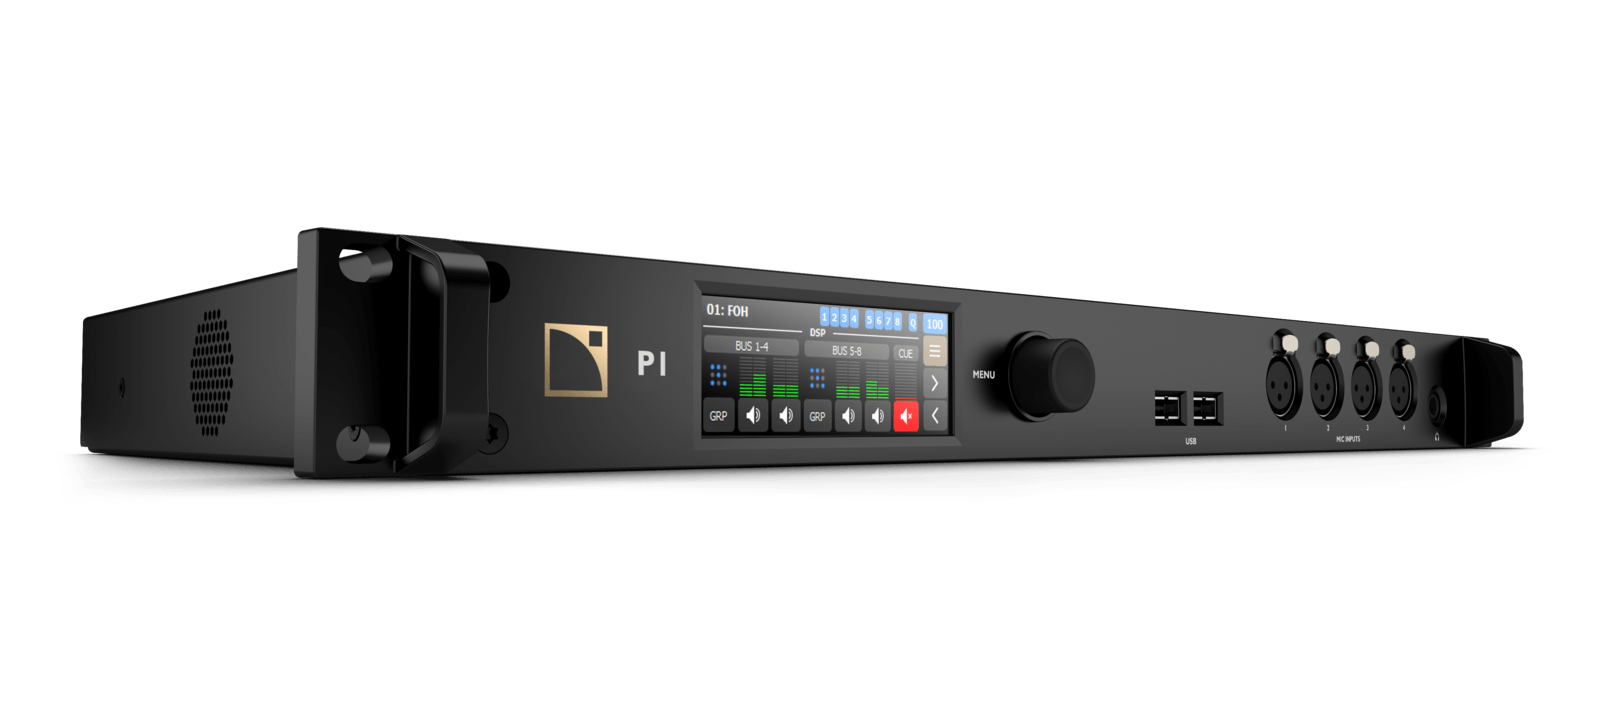
\includegraphics[width=\linewidth]{3DR_P1_Perspective.png}\\
\vfill
\normalsize Busse Lommers \\
Robin van den Dungen \\
Mahmud Gürler \\
Silas Kamphuis \\
Hein Verhallen \\
Youri Tils \\
Ahmed Abdelrahim \\
Fontys Hogescholen, De Rondom 1, 5612 AP Eindhoven \\
\today

\begin{justify}

\newpage
\tableofcontents
\thispagestyle{empty}

\listoffigures
\thispagestyle{empty}

\listoftables
\thispagestyle{empty}

\newpage
\pagestyle{plain}
\setcounter{page}{1}

\chapter{Introduction}
The project audio-DSP raises the main question: \textbf{"How to design an audio-DSP?"}. From the main research question the following sub-research questions are derived:

\begin{itemize}
\item What is the best method for creating digital filters?
\item What is the best method for creating digital effects?
\item What is the most suitable anti-aliasing filter?
\item What is the optimal needed roll-off for the anti-aliasing filter for a given bandwidth such that the noise can be negligible?
\item What is the minimum sample frequency needed to capture the desired frequency spectrum?
\item What is the minimum frequency range to be sampled to achieve sufficient detailed audio?
\item What is the lowest allowable noise for decent audio?
\item What ADC resolution is needed such that the quantization error and noise level are on par?
\item What ADC and DAC architecture is most suitable for this application?
\item What kind of processor is most suitable for this application?
\item What is the permittable jitter for accurate audio?
\item What is the maximum allowable ripple on the reference voltage for the ADC and DAC?
\item How much RAM does the system need?
\item How much flash does the system need?
\item What power supply topology is best suited for each part of the system?
\end{itemize}

\noindent \\In the following chapter the sub-research questions will be researched and documented.

\chapter{Research questions}

	\section{Best method for creating digital filters}	
		%%BACKGROUND
When listening to music it is of great importance that the speakers are tuned to the environment and the position of the listener. This is necessary to achieve the best experience. If the speakers are not correctly tuned to the surrounding environment, a digital signal processor (DSP) is used to correct this. A DSP is a specialized processor which is used for digital signal processing. 

In the audio world a DSP is used to optimize a sound system. For example some speakers have some imperfections and a DSP can be used to correct for these imperfections. It is also often used to add more dynamics to sound.

	\section{Best method for creating digital effects}
	
	\section{Most suitable anti-aliasing filter}
	
	\section{}

% Bibliography with heading so it pops up in the table of contents (idkwhy but this is how it works)
\printbibliography[
	heading=bibintoc,
	title={Bibliography}
]

\appendix

\chapter{Appendix A}

\end{justify}
\end{document}
